%%%%%%%%%%%%%%%%%%%%%%%%%%%%%%%%%%%%%%%%%
% Compact Laboratory Book
% LaTeX Template
% Version 1.0 (4/6/12)
%
% This template has been downloaded from:
% http://www.LaTeXTemplates.com
%
% Original author:
% Joan Queralt Gil (http://phobos.xtec.cat/jqueralt) using the labbook class by
% Frank Kuster (http://www.ctan.org/tex-archive/macros/latex/contrib/labbook/)
%
% License:
% CC BY-NC-SA 3.0 (http://creativecommons.org/licenses/by-nc-sa/3.0/)
%
% Important note:
% This template requires the labbook.cls file to be in the same directory as the
% .tex file. The labbook.cls file provides the necessary structure to create the
% lab book.
%
% The \lipsum[#] commands throughout this template generate dummy text
% to fill the template out. These commands should all be removed when 
% writing lab book content.
%
% HOW TO USE THIS TEMPLATE 
% Each day in the lab consists of three main things:
%
% 1. LABDAY: The first thing to put is the \labday{} command with a date in 
% curly brackets, this will make a new section showing that you are working
% on a new day.
%
% 2. EXPERIMENT/SUBEXPERIMENT: Next you need to specify what 
% experiment(s) and subexperiment(s) you are working on with a 
% \experiment{} and \subexperiment{} commands with the experiment 
% shorthand in the curly brackets. The experiment shorthand is defined in the 
% 'DEFINITION OF EXPERIMENTS' section below, this means you can 
% say \experiment{pcr} and the actual text written to the PDF will be what 
% you set the 'pcr' experiment to be. If the experiment is a one off, you can 
% just write it in the bracket without creating a shorthand. Note: if you don't 
% want to have an experiment, just leave this out and it won't be printed.
%
% 3. CONTENT: Following the experiment is the content, i.e. what progress 
% you made on the experiment that day.
%
%%%%%%%%%%%%%%%%%%%%%%%%%%%%%%%%%%%%%%%%%

%----------------------------------------------------------------------------------------
%	PACKAGES AND OTHER DOCUMENT CONFIGURATIONS
%----------------------------------------------------------------------------------------                               

\documentclass[fontsize=11pt, % Document font size
paper=a4, % Document paper type
twoside, % Shifts odd pages to the left for easier reading when printed, can be changed to oneside
captions=tableheading,
index=totoc,
hyperref]{labbook}

\usepackage[bottom=10em]{geometry} % Reduces the whitespace at the bottom of the page so more text can fit

\usepackage[english]{babel} % English language
\usepackage{lipsum} % Used for inserting dummy 'Lorem ipsum' text into the template

\usepackage[utf8]{inputenc} % Uses the utf8 input encoding
\usepackage[T1]{fontenc} % Use 8-bit encoding that has 256 glyphs

\usepackage[osf]{mathpazo} % Palatino as the main font
\linespread{1.05}\selectfont % Palatino needs some extra spacing, here 5% extra
\usepackage[scaled=.88]{beramono} % Bera-Monospace
\usepackage[scaled=.86]{berasans} % Bera Sans-Serif

\usepackage{booktabs,array} % Packages for tables

\usepackage{amsmath} % For typesetting math
\usepackage{graphicx} % Required for including images
\usepackage{etoolbox}
\usepackage[norule]{footmisc} % Removes the horizontal rule from footnotes
\usepackage{lastpage} % Counts the number of pages of the document
\usepackage{shadowtext}
\usepackage{minted}
\usepackage[backend=biber,
style=authoryear-comp,
natbib=true,
]{biblatex}
\addbibresource{JNMansfield_wk6StatusReport_10AUG13.bib}

\usepackage{setspace}
\usepackage{url}

\addtokomafont{title}{\Huge\color{green!40!brown!80}} % Titles in custom blue color
\addtokomafont{chapter}{\color{green!40!brown!80}} % Lab dates in olive green
\addtokomafont{section}{\color{brown}} % Sections in sepia
\addtokomafont{pagehead}{\normalfont\sffamily\color{gray}} % Header text in gray and sans serif
\addtokomafont{caption}{\footnotesize\itshape} % Small italic font size for captions
\addtokomafont{captionlabel}{\upshape\bfseries} % Bold for caption labels
\addtokomafont{descriptionlabel}{\rmfamily}
\setcapwidth[r]{10cm} % Right align caption text
\setkomafont{footnote}{\sffamily} % Footnotes in sans serif

\deffootnote[4cm]{4cm}{1em}{\textsuperscript{\thefootnotemark}} % Indent footnotes to line up with text

\DeclareFixedFont{\textcap}{T1}{phv}{bx}{n}{1.5cm} % Font for main title: Helvetica 1.5 cm
\DeclareFixedFont{\textaut}{T1}{phv}{bx}{n}{0.8cm} % Font for author name: Helvetica 0.8 cm

\usepackage[nouppercase,headsepline]{scrpage2} % Provides headers and footers configuration
\pagestyle{scrheadings} % Print the headers and footers on all pages
\clearscrheadfoot % Clean old definitions if they exist

\automark[chapter]{chapter}
\ohead{\headmark} % Prints outer header

\setlength{\headheight}{25pt} % Makes the header take up a bit of extra space for aesthetics
\setheadsepline{.4pt} % Creates a thin rule under the header
\addtokomafont{headsepline}{\color{lightgray}} % Colors the rule under the header light gray

\ofoot[\normalfont\normalcolor{\thepage\ |\  \pageref{LastPage}}]{\normalfont\normalcolor{\thepage\ |\  \pageref{LastPage}}} % Creates an outer footer of: "current page | total pages"

% These lines make it so each new lab day directly follows the previous one i.e. does not start on a new page - comment them out to separate lab days on new pages
\makeatletter
\patchcmd{\addchap}{\if@openright\cleardoublepage\else\clearpage\fi}{\par}{}{}
\makeatother
\renewcommand*{\chapterpagestyle}{scrheadings}


% These lines make it so every figure and equation in the document is numbered consecutively rather than restarting at 1 for each lab day - comment them out to remove this behavior
\usepackage{chngcntr}
\counterwithout{figure}{labday}
\counterwithout{equation}{labday}

% Hyperlink configuration
\usepackage[
pdfauthor={}, % Your name for the author field in the PDF
pdftitle={Laboratory Journal}, % PDF title
pdfsubject={}, % PDF subject
bookmarksopen=true,
linktocpage=true,
pdfpagelabels=true,
plainpages=false,
colorlinks=true, % Turn off all coloring by changing this to false
bookmarks=true,
pdfview=FitB]{hyperref}

\usepackage[stretch=10]{microtype} % Slightly tweak font spacing for aesthetics

%\setlength\parindent{0pt} % Uncomment to remove all indentation from paragraphs

%----------------------------------------------------------------------------------------
%	DEFINITION OF EXPERIMENTS
%----------------------------------------------------------------------------------------

% Template: \newexperiment{<abbrev>}[<short form>]{<long form>}
% <abbrev> is the reference to use later in the .tex file in \experiment{}, the <short form> is only used in the table of contents and running title - it is optional, <long form> is what is printed in the lab book itself

\newexperiment{exp1}[A Second Database]{The need for a Second Database}
\newexperiment{exp2}[Exploring UI possibilities]{Some exploration of UI possibilities}
\newexperiment{exp3}[Fragments] {An attempt to use a fragment}


%----------------------------------------------------------------------------------------

\begin{document}

%----------------------------------------------------------------------------------------
%	TITLE PAGE
%----------------------------------------------------------------------------------------

\title{\textcap{\shadowtext{CS493}\\
\textaut{\small{Regis University}}	
\textaut{\small{Senior Capstone}}\\		
\textaut{\shadowtext{Week Six}}}
}

\author{

\includegraphics[scale=0.5]{android.png}\\
\textaut{\small{Intructor: Mr. Allan Rossi}}\\
\textaut{\small{Author: Mr. Jason N Mansfield}}\\ \\ % Your name
The Object Based Study Application % Your degree
}
\date{\today} % No date by default, add \today if you wish to include the publication date

\maketitle % Title page

\printindex
\tableofcontents % Table of contents
\newpage % Start lab look on a new page


\pagestyle{scrheadings} % Begin using headers

%----------------------------------------------------------------------------------------
%	LAB BOOK CONTENTS
%----------------------------------------------------------------------------------------

\labday{\today}
%-----------------------------------------

\experiment{exp1}
\begin{onehalfspace}
I have reached a point in this project where I feel far more comfortable with the Android API. I have been able to grasp a few of the basic concepts related to the SQLite database, Fragments, Adapters, Cursors and other interesting elements. After I finally achieved adding and removing data to the database while updating the ListView~\citep{listview}, I suddenly realized I would need a second database to expand an additional branch of content. Therefore, I now have two SQLite databases which are now functional. I am still trying to decide how to approach the final view which is to offer the user a look at their stored information so to speak. As it stands now the user creates a Object and associated description. This information is stored in the first database created~\citep{sqlite}:
\end{onehalfspace}
\begin{minted}[fontsize=\scriptsize]{java}
public class DatabaseH extends SQLiteOpenHelper{

private SQLiteDatabase sqLiteDatabase;

private static final int DATABASE_VER = 1;
private static final String DATABASE_NAME = "learning";
//table columns

public static final class KEYS implements BaseColumns{
private KEYS() {}
public static final String TABLE_NAME = "objects";
public static final String KEY_ID = "_id";
public static final String KEY_OBNAME = "objectName";
public static final String KEY_CONTENT = "content";
public DatabaseH(Context context){
super(context, DATABASE_NAME, null, DATABASE_VER);
}
//Creating Tables
@Override
public void onCreate(SQLiteDatabase db){
db.execSQL("DROP TABLE IF EXISTS " + KEYS.TABLE_NAME);
String CREATE_OBJECT_TABLE = "CREATE TABLE " + KEYS.TABLE_NAME + "("
+ KEYS.KEY_ID + " INTEGER PRIMARY KEY," + KEYS.KEY_OBNAME + " TEXT,"
+ KEYS.KEY_CONTENT+ " TEXT" + ")";
db.execSQL(CREATE_OBJECT_TABLE);
}
}
\end{minted}
\clearpage
\begin{onehalfspace}
Similarly, the newer database is designed to hold an id, title of sorts and then related content:
\end{onehalfspace}
\begin{minted}[fontsize=\scriptsize]{java}
public class DatabaseTwo extends SQLiteOpenHelper
{
private SQLiteDatabase sqLiteDatabase;

private static final int DATABASE_VER = 1;
private static final String DATABASE_NAME = "griddatabase";
//table columns

public static final class CUBES implements BaseColumns {
private CUBES() {}
public static final String TABLE_NAME = "gridtable";
public static final String KEY_ID = "_id";
public static final String KEY_OBNAME = "cubename";
public static final String KEY_CONTENT = "cube";
}
public DatabaseTwo(Context context){
super(context, DATABASE_NAME, null, DATABASE_VER);
}
//Creating Tables
@Override
public void onCreate(SQLiteDatabase db){
db.execSQL("DROP TABLE IF EXISTS " + CUBES.TABLE_NAME);
String CREATE_OBJECT_TABLE = "CREATE TABLE " + CUBES.TABLE_NAME + "("
+ CUBES.KEY_ID + " INTEGER PRIMARY KEY," + CUBES.KEY_OBNAME + " TEXT,"
+ CUBES.KEY_CONTENT+ " TEXT" + ")";
db.execSQL(CREATE_OBJECT_TABLE);
}
\end{minted}

\experiment{exp2}
\begin{onehalfspace}
Having accomplished a ListView and arriving closer to the End Game, for this particular project, the need for aesthetics is becoming a issue. The current application is not entirely hideous, but it is not pleasing to the eye by any stretch of the imagination. I attempted to create a GridView~\citep{gridview} at first but it appeared to make the current layout more cluttered then anything. Had I taken a different approach earlier it may have been useful? The final look of the application will unlikely be memorable but at this point, with the amount of time I have remaining, I believe I will shoot for functional and clean. The following image shows a child of the object with its title and description. On top is a Fragment which may or may not be used in the final product to contain a second ListView. 
\end{onehalfspace}
\begin{center}
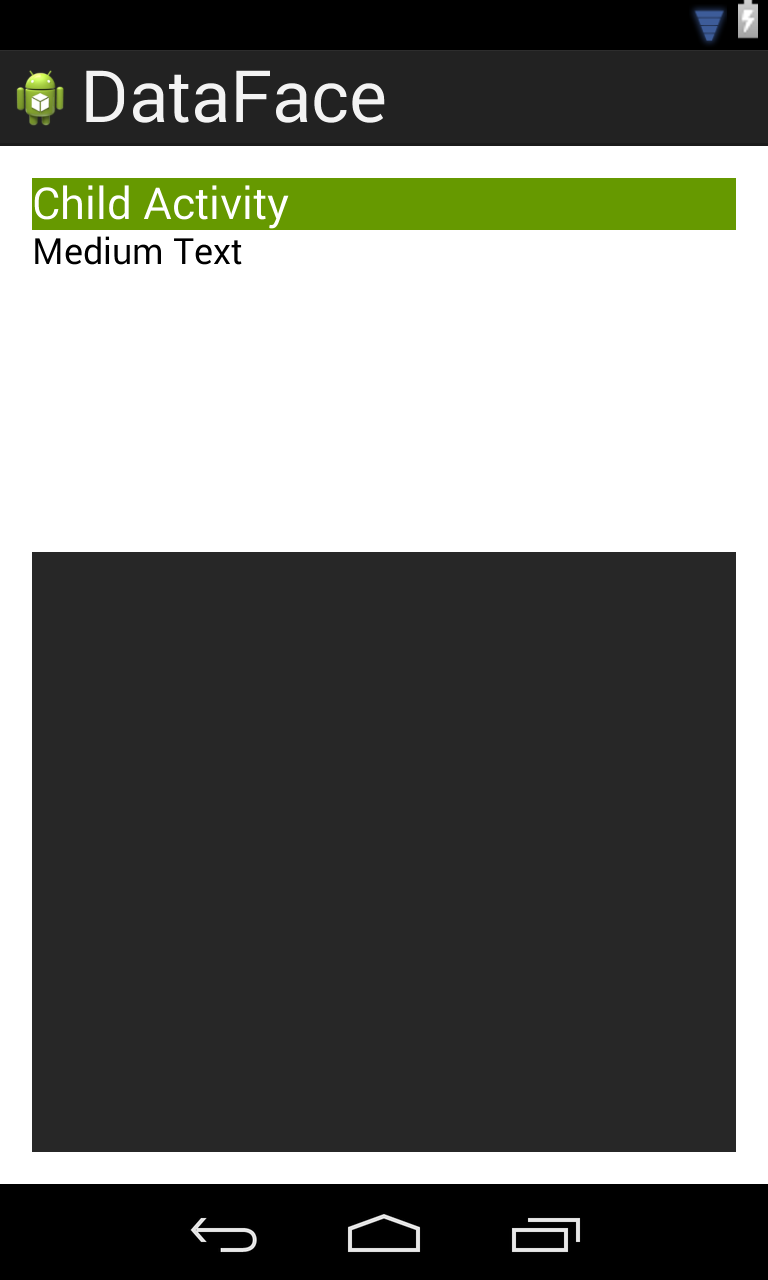
\includegraphics[scale=0.2]{UI.png}
\end{center}
\experiment{exp3}
\begin{onehalfspace}
	I have had more success this week with using Fragments~\citep{fragments} and I feel its time to try and implement one for the final View. This will allow me to expand this application in the future as I can simply swap out Fragments as opposed to completely re-writing an entire Activity. Fragments can make matters more complex, but in many ways they appear to add enough scalability that they are a more than fair trade for running an additional Activity:
\end{onehalfspace}
\begin{minted}[fontsize=\scriptsize]{xml}
<FrameLayout android:name="com.beta.dataface.ObjectFragment"
android:id="@+id/fragment_container"
android:layout_alignParentBottom="true"
android:layout_width="match_parent"
android:layout_height="300dp"
android:background="#D8000000"
tools:layout="@layout/child_activity"/>
\end{minted}
\begin{onehalfspace}
My only regret is that I do not have more time to expand this particular application to show for my senior capstone. Although, my intentions are to continue working on this particular application until its fully functional. My goal is to have the basic needs met by the middle of next week, such as data entry for the user to both databases, and an understandable TextView for them to later review this data. The deletion feature and first ListView are already accomplished.
\end{onehalfspace}
\clearpage
\printbibliography

\end{document}
